\chapter{Anhang}
\label{a:append}
\section*{Abbildungen}

\begin{figure}[H]
	\centering
	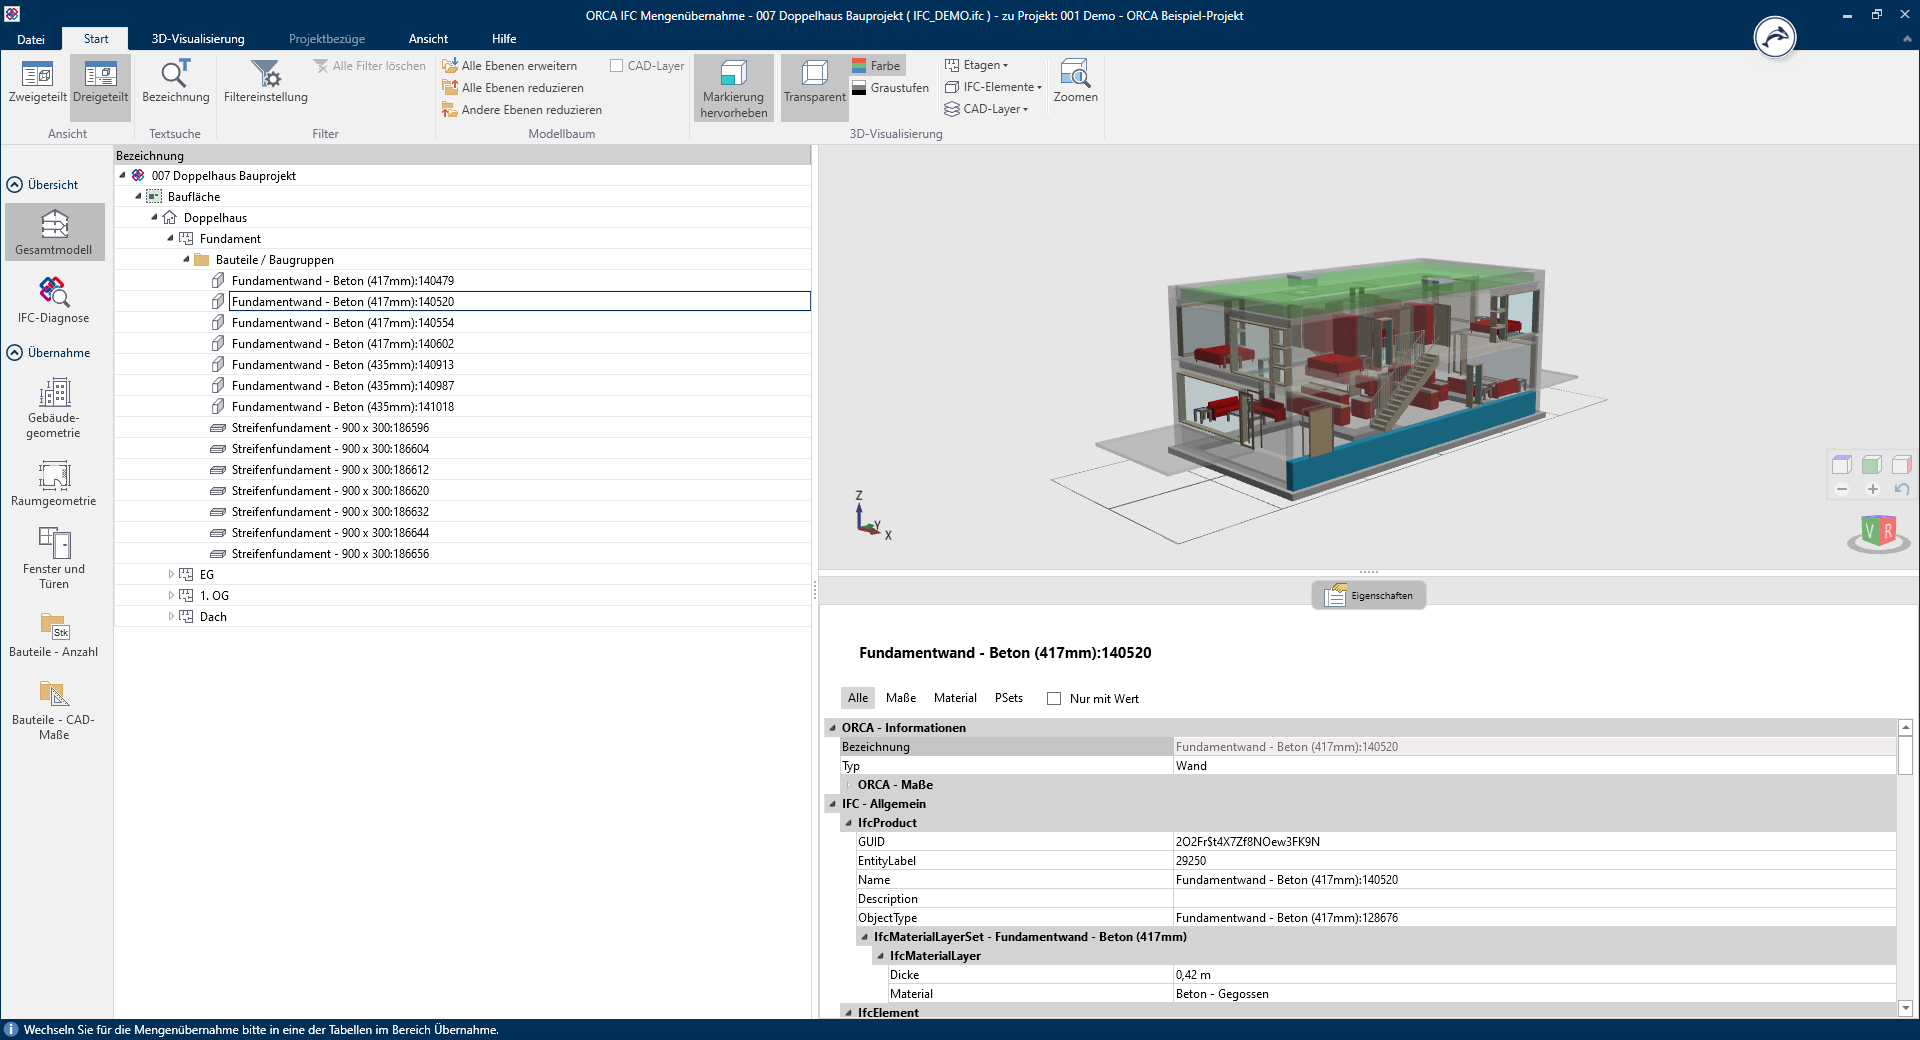
\includegraphics[width=1\linewidth]{ifc-manager}
	\caption[IFC Manager]{Oberfläche des \ac{ifc} Manager}
	\label{fig:ifc-manager}
\end{figure}

\begin{figure}[H]
	\centering
	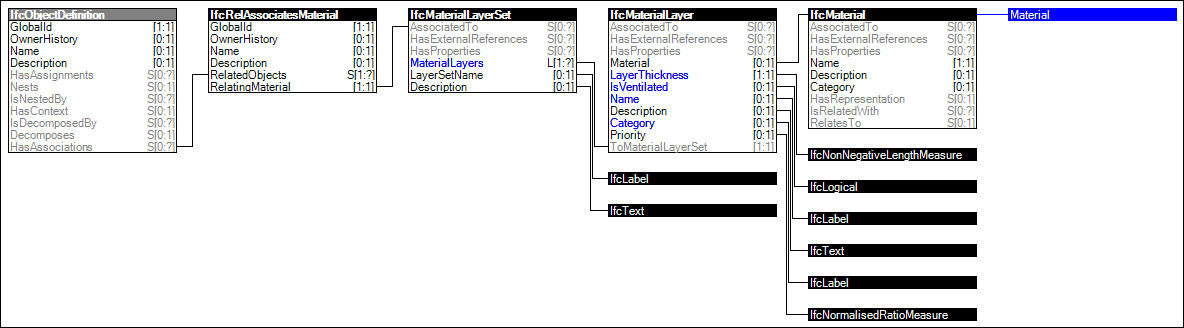
\includegraphics[width=1\linewidth]{material-layer-set}
	\caption[IfcMaterialLayerSet]{Material Layer Set Association}
	\label{fig:layer-set}
\end{figure}

\begin{sidewaysfigure}
	\centering
	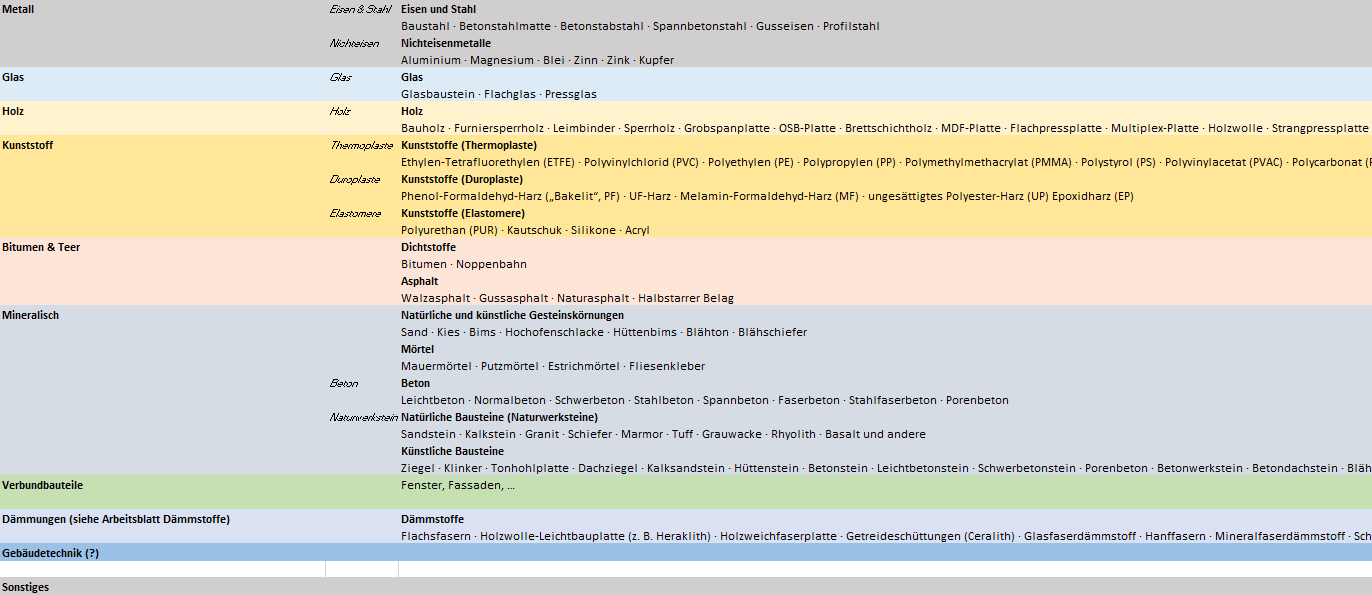
\includegraphics[width=\textheight]{material-categories}
	\caption[MaterialCategories]{Überkategorien für die Klassifizierung von Materialien mit Beispielen}
	\label{fig:material-categories}
\end{sidewaysfigure}

\begin{figure}[H]
	\centering
	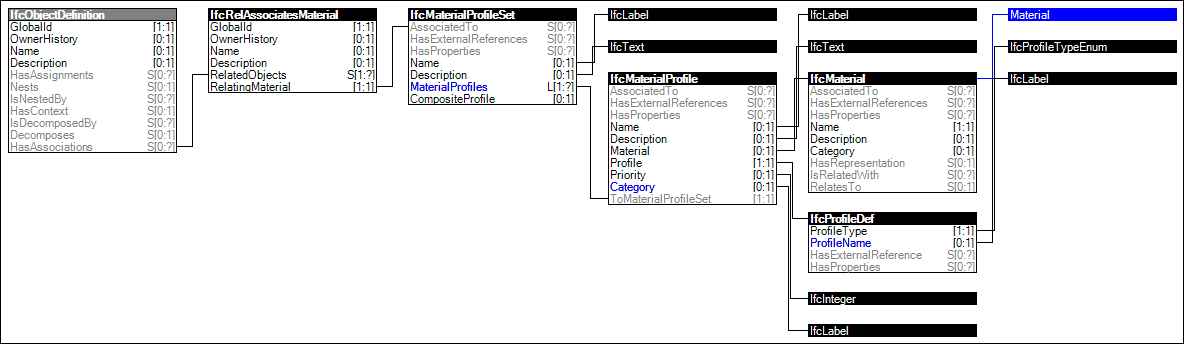
\includegraphics[width=1\linewidth]{material-profile-set}
	\caption[IfcMaterialProfileSet]{Material Profile Set Association}
	\label{fig:profile-set}
\end{figure}

\begin{figure}[H]
	\centering
	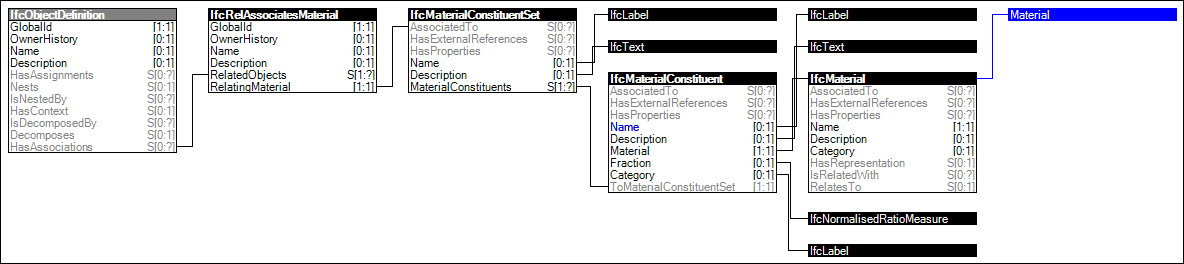
\includegraphics[width=1\linewidth]{material-constituent-set}
	\caption[IfcMaterialConsituentSet]{Material Constituent Set Association}
	\label{fig:constituent-set}
\end{figure}

\begin{figure}[H]
	\centering
	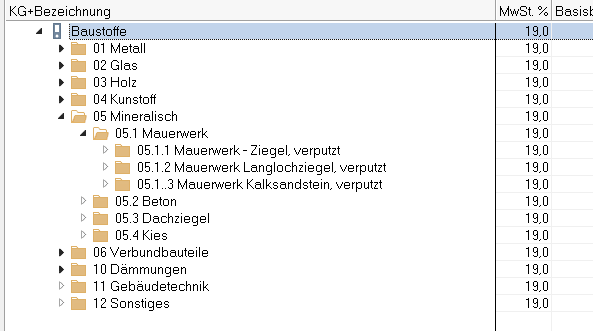
\includegraphics[width=1\linewidth]{cost-structure-example}
	\caption[CostStructure]{Beispiel einer Kostengliederung in der ORCA AVA}
	\label{fig:cost-structure}
\end{figure}

\begin{figure}[H]
	\centering
	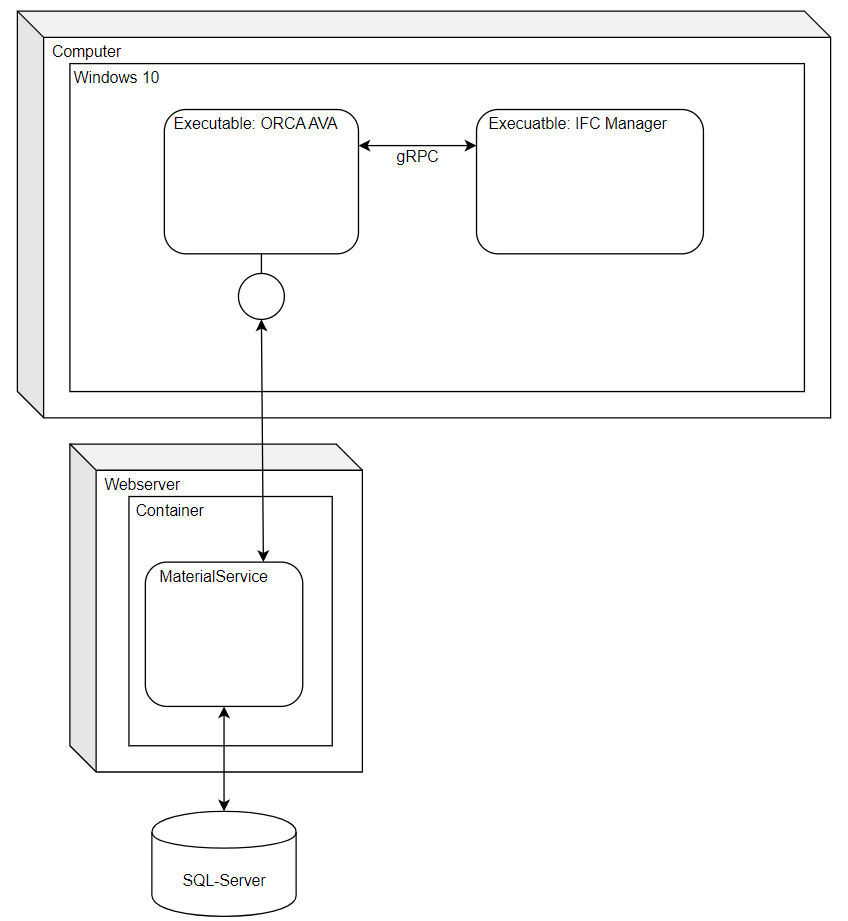
\includegraphics[width=1\linewidth]{verteilungsdiagramm}
	\caption[Verteilungsdiagramm]{Verteilungsdiagramm der Architektur}
	\label{fig:distribution-diagramm}
\end{figure}

\begin{figure}[H]
	\centering
	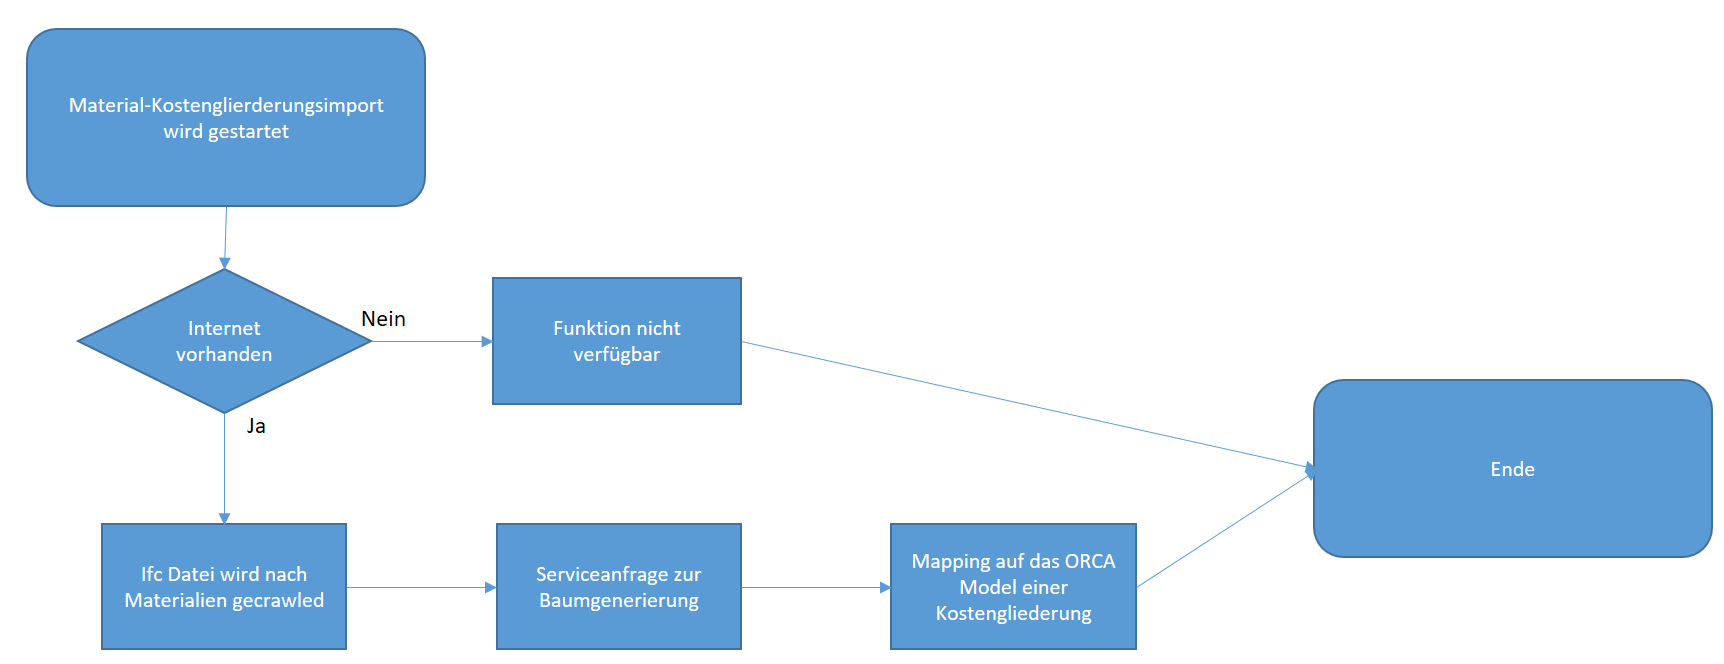
\includegraphics[width=1\linewidth]{function-import}
	\caption[Import]{Flussdiagramm Import der Material-Kostengliederung}
	\label{fig:func-import}
\end{figure}

\begin{figure}[H]
	\centering
	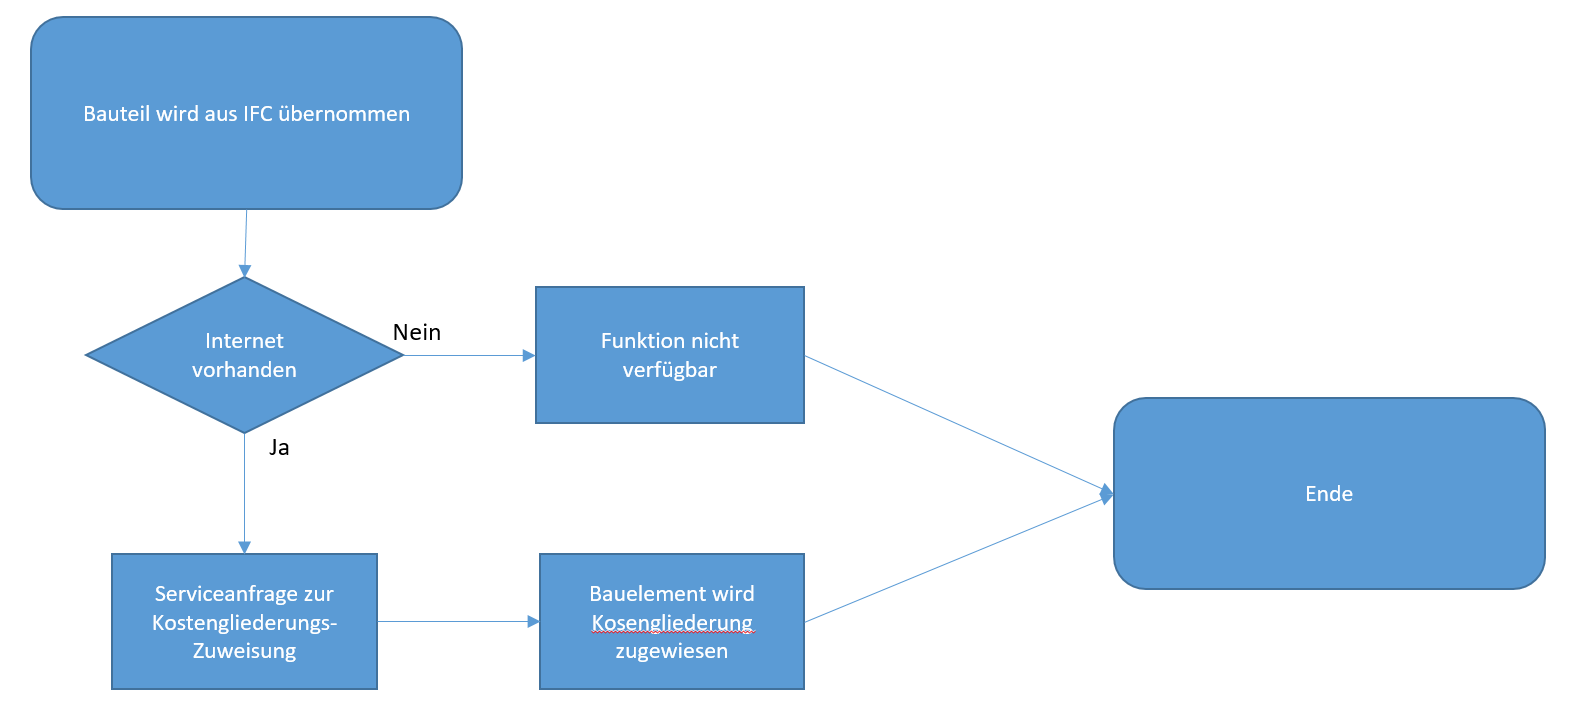
\includegraphics[width=1\linewidth]{function-takeover}
	\caption[Takeover]{Flussdiagramm Übernahme von Mengen aus dem \ac{ifc} Manager}
	\label{fig:func-takeover}
\end{figure}

\begin{figure}[H]
	\centering
	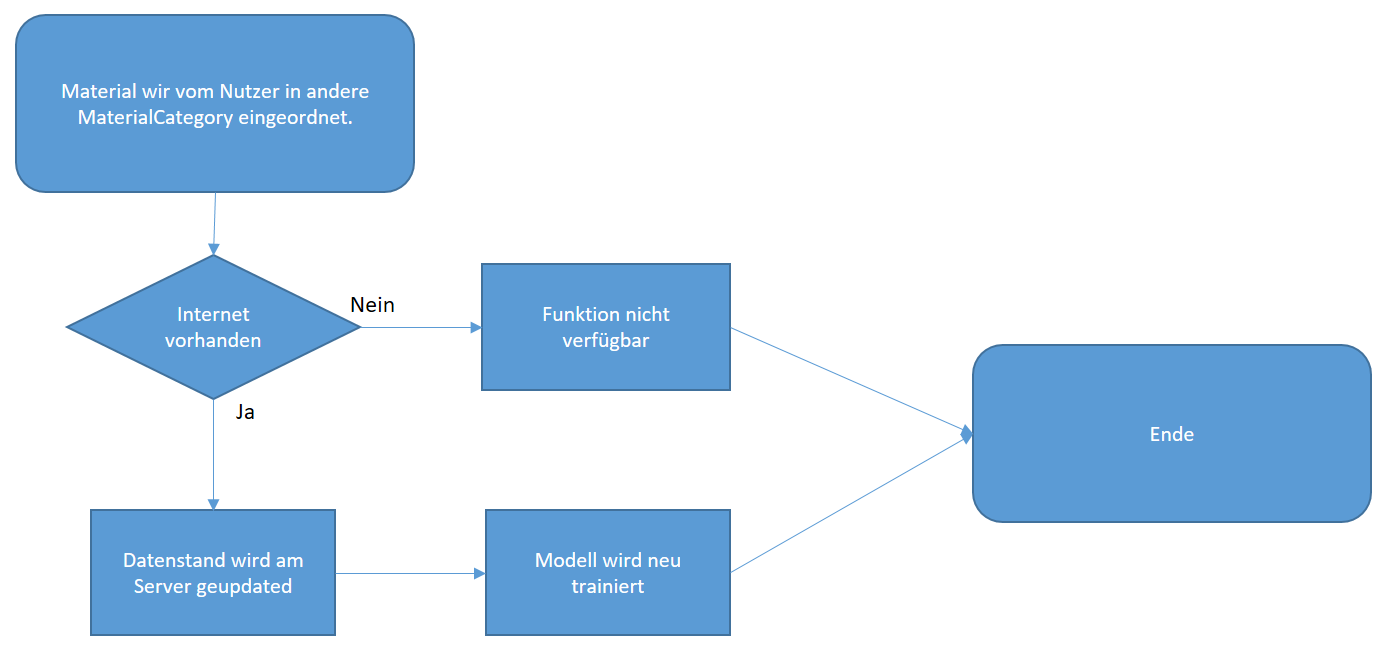
\includegraphics[width=1\linewidth]{function-rating}
	\caption[Rating]{Flussdiagramm Bewertung des Kostengliederungs-Import}
	\label{fig:func-rating}
\end{figure}

\begin{figure}[H]
	\centering
	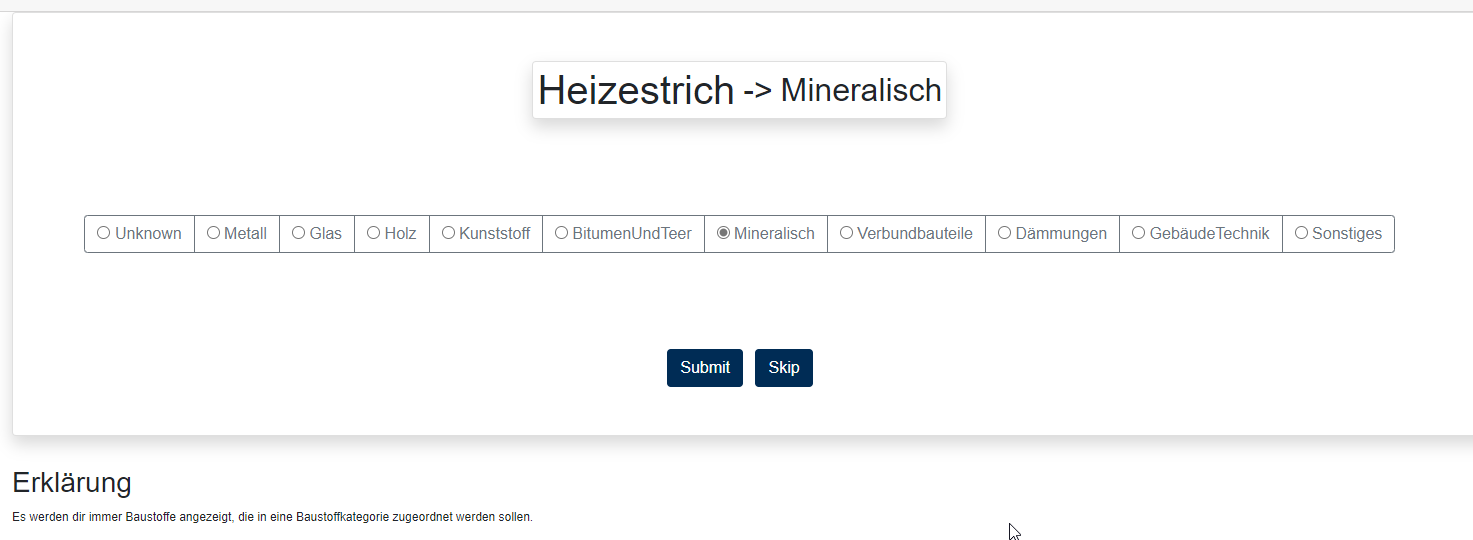
\includegraphics[width=1\linewidth]{material-classifier-gui}
	\caption[Rating]{Oberfläche des Klassifizierungs-Tools für Materialien}
	\label{fig:classification-service}
\end{figure}

\begin{figure}[H]
	\centering
	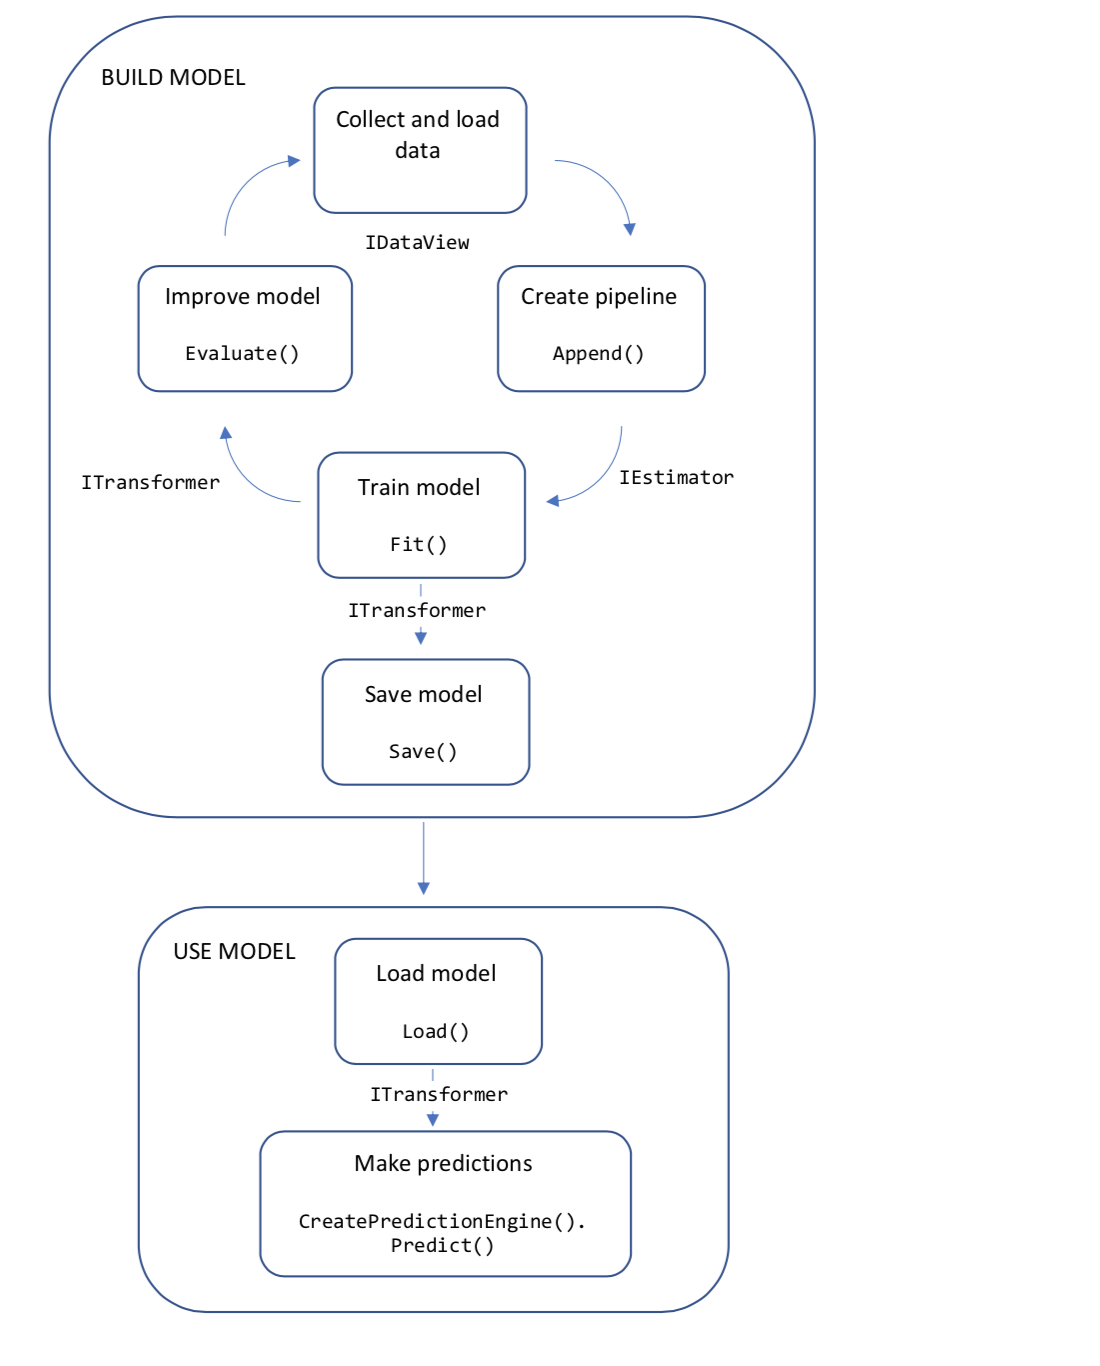
\includegraphics[width=\textwidth]{mldotnet-workflow}
	\caption[CBOW]{Code Workflow von \textit{ML.NET} (Quelle:  \cite{mlnet2022})}
	\label{fig:mlnet-workflow}
\end{figure}


\newpage
\section*{Listings}
\label{c:listings}

\lstinputlisting[language={[Sharp]C}, caption={Implementierung der Methode \code{GenerateMaterialCostStructureAsync} der Klasse \code{MateialService}}, style={csharp}, label={lst:materialservice}]{MaterialService.cs}

\lstinputlisting[language={[Sharp]C}, caption={Python-Interopt für das Preprocessing}, style={csharp}, label={lst:python-preprocess}]{PythonPreprocess.cs}

\lstinputlisting[language={python}, caption={Python-Interopt für das Preprocessing}, label={Script}, label={lst:preprocess}]{preprocess.py}

\newpage
\section*{Tabellen}
\label{c:tables}
\begin{table}[!ht]
	\centering
	\resizebox{\columnwidth}{!}{						
	     \begin{tabular}{|l|l|l|l|l|l|l|l|l|l|l|l|l|l|}
	    	\hline
	    	\textbf{Predicted ->} & \textbf{} & \textbf{0} & \textbf{1} & \textbf{2} & \textbf{3} & \textbf{4} & \textbf{5} & \textbf{6} & \textbf{7} & \textbf{8} & \textbf{9} & \textbf{} & \textbf{Recall} \\ \hline
	    	\textbf{Truth} & ~ & ~ & ~ & ~ & ~ & ~ & ~ & ~ & ~ & ~ & ~ & ~ & ~ \\ \hline
	    	\textbf{Mineralisch } & ~ & 22 & 0 & 0 & 0 & 0 & 2 & 0 & 0 & 0 & 0 & ~ & 0,9167 \\ \hline
	    	\textbf{Sonstiges } & ~ & 4 & 8 & 0 & 0 & 0 & 0 & 0 & 0 & 0 & 0 & ~ & 0,6667 \\ \hline
	    	\textbf{Dämmungen} & ~ & 0 & 0 & 7 & 0 & 0 & 0 & 0 & 0 & 0 & 0 & ~ & 1,0000 \\ \hline
	    	\textbf{Holz } & ~ & 0 & 0 & 0 & 7 & 0 & 0 & 0 & 0 & 0 & 0 & ~ & 1,0000 \\ \hline
	    	\textbf{Verbundbauteile } & ~ & 1 & 0 & 0 & 0 & 5 & 0 & 0 & 1 & 0 & 0 & ~ & 0,7143 \\ \hline
	    	\textbf{Metall } & ~ & 2 & 1 & 0 & 0 & 0 & 25 & 0 & 0 & 0 & 0 & ~ & 0,8929 \\ \hline
	    	\textbf{Kunststoff } & ~ & 0 & 0 & 0 & 0 & 0 & 0 & 4 & 0 & 0 & 0 & ~ & 1,0000 \\ \hline
	    	\textbf{Glas } & ~ & 0 & 0 & 0 & 0 & 0 & 0 & 0 & 4 & 0 & 0 & ~ & 1,0000 \\ \hline
	    	\textbf{GebäudeTechnik } & ~ & 0 & 0 & 0 & 0 & 0 & 0 & 0 & 0 & 1 & 0 & ~ & 1,0000 \\ \hline
	    	\textbf{BitumenUndTeer } & ~ & 0 & 0 & 0 & 0 & 0 & 0 & 0 & 0 & 0 & 0 & ~ & 0,0000 \\ \hline
	    	\textbf{} & ~ & ~ & ~ & ~ & ~ & ~ & ~ & ~ & ~ & ~ & ~ & ~ & ~ \\ \hline
	    	\textbf{Precision} & ~ & 0,7586  & 0,8889  & 1,0000 & 1,0000 & 1,0000 & 0,9259  & 1,0000 & 0,8000  & 1,0000 & 0,0000 & ~ & ~ \\ \hline
	    \end{tabular}
	}
	\caption{Konfusionsmatrix: ScdaMaximumEntropy}
	\label{t:confusionmatrix-sdca}
\end{table}

\begin{table}[!ht]
	\centering
	\resizebox{\columnwidth}{!}{		
		\begin{tabular}{|l|l|l|l|l|l|l|l|l|l|l|l|l|l|}
			\hline
			\textbf{Predicted ->} & \textbf{} & \textbf{0} & \textbf{1} & \textbf{2} & \textbf{3} & \textbf{4} & \textbf{5} & \textbf{6} & \textbf{7} & \textbf{8} & \textbf{9} & \textbf{} & \textbf{Recall} \\ \hline
			\textbf{Truth} & ~ & ~ & ~ & ~ & ~ & ~ & ~ & ~ & ~ & ~ & ~ & ~ & ~ \\ \hline
			\textbf{0. Mineralisch} & ~ & 23 & 0 & 0 & 0 & 0 & 1 & 0 & 0 & 0 & 0 & ~ & 0,9583 \\ \hline
			\textbf{1. Sonstiges } & ~ & 9 & 3 & 0 & 0 & 0 & 0 & 0 & 0 & 0 & 0 & ~ & 0,2500 \\ \hline
			\textbf{2. Dämmungen} & ~ & 4 & 0 & 3 & 0 & 0 & 0 & 0 & 0 & 0 & 0 & ~ & 0,4286 \\ \hline
			\textbf{3. Holz } & ~ & 1 & 0 & 0 & 6 & 0 & 0 & 0 & 0 & 0 & 0 & ~ & 0,8571 \\ \hline
			\textbf{4. Verbundbauteile } & ~ & 4 & 0 & 0 & 0 & 3 & 0 & 0 & 0 & 0 & 0 & ~ & 0,4286 \\ \hline
			\textbf{5. Metall } & ~ & 10 & 0 & 0 & 0 & 0 & 18 & 0 & 0 & 0 & 0 & ~ & 0,6429 \\ \hline
			\textbf{6. Kunststoff } & ~ & 1 & 0 & 0 & 0 & 0 & 0 & 3 & 0 & 0 & 0 & ~ & 0,7500 \\ \hline
			\textbf{7. Glas } & ~ & 0 & 0 & 0 & 0 & 0 & 0 & 0 & 4 & 0 & 0 & ~ & 1,0000 \\ \hline
			\textbf{8. GebäudeTechnik } & ~ & 1 & 0 & 0 & 0 & 0 & 0 & 0 & 0 & 0 & 0 & ~ & 0,0000 \\ \hline
			\textbf{9. BitumenUndTeer } & ~ & 0 & 0 & 0 & 0 & 0 & 0 & 0 & 0 & 0 & 0 & ~ & 0,0000 \\ \hline
			\textbf{} & ~ & ~ & ~ & ~ & ~ & ~ & ~ & ~ & ~ & ~ & ~ & ~ & ~ \\ \hline
			\textbf{Precision} & ~ & 0,4340  & 1,0000 & 1,0000 & 1,0000 & 1,0000 & 0,9474  & 1,0000 & 1,0000 & 0,0000 & 0,0000 & ~ & ~ \\ \hline
		\end{tabular}
	}
	\caption{Konfusionsmatrix: LbfgsMaximumEntorpy}
	\label{t:confusionmatrix-lbfgs}
\end{table}

\begin{table}[!ht]
	\centering
	\resizebox{\columnwidth}{!}{		
		\begin{tabular}{|l|l|l|l|l|l|l|l|l|l|l|l|l|l|}
			\hline
			\textbf{Predicted ->} & \textbf{} & \textbf{0} & \textbf{1} & \textbf{2} & \textbf{3} & \textbf{4} & \textbf{5} & \textbf{6} & \textbf{7} & \textbf{8} & \textbf{9} & \textbf{} & \textbf{Recall} \\ \hline
			\textbf{Truth} & ~ & ~ & ~ & ~ & ~ & ~ & ~ & ~ & ~ & ~ & ~ & ~ & ~ \\ \hline
			\textbf{0. Mineralisch} & ~ & 22 & 0 & 0 & 0 & 0 & 2 & 0 & 0 & 0 & 0 & ~ & 0,9167 \\ \hline
			\textbf{1. Sonstiges } & ~ & 4 & 8 & 0 & 0 & 0 & 0 & 0 & 0 & 0 & 0 & ~ & 0,6667 \\ \hline
			\textbf{2. Dämmungen} & ~ & 0 & 0 & 7 & 0 & 0 & 0 & 0 & 0 & 0 & 0 & ~ & 1,0000 \\ \hline
			\textbf{3. Holz } & ~ & 0 & 0 & 0 & 7 & 0 & 0 & 0 & 0 & 0 & 0 & ~ & 1,0000 \\ \hline
			\textbf{4. Verbundbauteile } & ~ & 1 & 0 & 0 & 0 & 4 & 1 & 0 & 1 & 0 & 0 & ~ & 0,5714 \\ \hline
			\textbf{5. Metall } & ~ & 2 & 1 & 0 & 0 & 0 & 25 & 0 & 0 & 0 & 0 & ~ & 0,8929 \\ \hline
			\textbf{6. Kunststoff } & ~ & 0 & 0 & 0 & 0 & 0 & 0 & 4 & 0 & 0 & 0 & ~ & 1,0000 \\ \hline
			\textbf{7. Glas } & ~ & 0 & 0 & 0 & 0 & 0 & 0 & 0 & 4 & 0 & 0 & ~ & 1,0000 \\ \hline
			\textbf{8. GebäudeTechnik } & ~ & 0 & 0 & 0 & 0 & 0 & 0 & 0 & 0 & 1 & 0 & ~ & 1,0000 \\ \hline
			\textbf{9. BitumenUndTeer } & ~ & 0 & 0 & 0 & 0 & 0 & 0 & 0 & 0 & 0 & 0 & ~ & 0,0000 \\ \hline
			\textbf{} & ~ & ~ & ~ & ~ & ~ & ~ & ~ & ~ & ~ & ~ & ~ & ~ & ~ \\ \hline
			\textbf{Precision} & ~ & 0,7586  & 0,8889  & 1,0000 & 1,0000 & 1,0000 & 0,8929  & 1,0000 & 0,8000  & 1,0000 & 0,0000 & ~ & ~ \\ \hline
		\end{tabular}
	}
	\caption{Konfusionsmatrix: OneVersusAll}
	\label{t:confusionmatrix-onevsall}
\end{table}

\begin{table}[!ht]
	\label{key}
	\centering
	\resizebox{\columnwidth}{!}{		
		\begin{tabular}{|l|l|l|l|l|l|l|l|l|l|l|l|l|l|}
			\hline
			\textbf{Predicted ->} & \textbf{} & \textbf{0} & \textbf{1} & \textbf{2} & \textbf{3} & \textbf{4} & \textbf{5} & \textbf{6} & \textbf{7} & \textbf{8} & \textbf{9} & \textbf{} & \textbf{Recall} \\ \hline
			\textbf{Truth} & ~ & ~ & ~ & ~ & ~ & ~ & ~ & ~ & ~ & ~ & ~ & ~ & ~ \\ \hline
			\textbf{0. Mineralisch} & ~ & 21 & 0 & 0 & 0 & 0 & 3 & 0 & 0 & 0 & 0 & ~ & 0,8750 \\ \hline
			\textbf{1. Sonstiges } & ~ & 6 & 3 & 0 & 0 & 0 & 3 & 0 & 0 & 0 & 0 & ~ & 0,2500 \\ \hline
			\textbf{2. Dämmungen} & ~ & 7 & 0 & 0 & 0 & 0 & 0 & 0 & 0 & 0 & 0 & ~ & 0,0000 \\ \hline
			\textbf{3. Holz } & ~ & 5 & 0 & 0 & 1 & 0 & 1 & 0 & 0 & 0 & 0 & ~ & 0,1429 \\ \hline
			\textbf{4. Verbundbauteile } & ~ & 6 & 0 & 0 & 0 & 0 & 1 & 0 & 0 & 0 & 0 & ~ & 0,0000 \\ \hline
			\textbf{5. Metall } & ~ & 11 & 0 & 0 & 0 & 0 & 17 & 0 & 0 & 0 & 0 & ~ & 0,6071 \\ \hline
			\textbf{6. Kunststoff } & ~ & 1 & 0 & 0 & 0 & 0 & 0 & 3 & 0 & 0 & 0 & ~ & 0,7500 \\ \hline
			\textbf{7. Glas } & ~ & 2 & 0 & 0 & 0 & 0 & 2 & 0 & 0 & 0 & 0 & ~ & 0,0000 \\ \hline
			\textbf{8. GebäudeTechnik } & ~ & 1 & 0 & 0 & 0 & 0 & 0 & 0 & 0 & 0 & 0 & ~ & 0,0000 \\ \hline
			\textbf{9. BitumenUndTeer } & ~ & 0 & 0 & 0 & 0 & 0 & 0 & 0 & 0 & 0 & 0 & ~ & 0,0000 \\ \hline
			\textbf{} & ~ & ~ & ~ & ~ & ~ & ~ & ~ & ~ & ~ & ~ & ~ & ~ & ~ \\ \hline
			\textbf{Precision} & ~ & 0,3500  & 1,0000  & 0,0000  & 1,0000 & 0,0000   & 0,6296  & 1,0000 & 0,0000 & 0,0000 & 0,0000 & ~ & ~ \\ \hline
		\end{tabular}
	}
	\caption{Konfusionsmatrix: TextclassificationersusAll}
	\label{t:confusionmatrix-text}
\end{table}
\begin{table}[h]

	\centering
\begin{tabular}{|l|l|l|l|}
	\hline
	\textbf{Begriff} & \textbf{Erwartet} & \textbf{DBSCAN} & \textbf{OpenAI}\\ \hline
   Ortbeton C30/37 Verputzt & 1 & 1 & ~ \\ \hline
Trockenbau Gipsplatte & ~ & ~ & ~ \\ \hline
Fußboden Heizestrich & 3 & 3 & 3 \\ \hline
Geländearbeiten Gebundene Schüttung & 4 & 4 & 4 \\ \hline
Ortbeton C30/37 & 1 & 1 & ~ \\ \hline
Mauerwerk mit Daemmeigenschaften & 2 & 2 & 2 \\ \hline
Fußboden Fußbodenaufbau & 3 & 3 & 3 \\ \hline
Fußboden Schüttung & 3 & ~ & 3 \\ \hline
Putz & ~ & ~ & ~ \\ \hline
Geländearbeiten Rollierung Schuettung & 4 & 4 & 4 \\ \hline
Ortbeton bewehrt geschliffen & 1 & ~ & ~ \\ \hline
Geländearbeiten Aufgeschüttet & 4 & 4 & 4 \\ \hline
Fußboden Estrich & 3 & 3 & 3 \\ \hline
Beton C 25/30 & 1 & 1 & ~ \\ \hline
Dachdeckung Ziegel & ~ & ~ & ~ \\ \hline
Mauerwerk ohne Daemmeigenschaften & 2 & 2 & 2 \\ \hline
\textbf{Auswertung} & richtig & teilweise & teilweise \\ \hline
	\end{tabular}
	\caption{Evaluationsbeispiel 1 (Überkategorie: Mineralisch)}
	\label{t:evaluation-example1}
\end{table}

\begin{table}[h]
	
	\centering
	\begin{tabular}{|l|l|l|l|}
		\hline
		\textbf{Begriff} & \textbf{Erwartet} & \textbf{DBSCAN} & \textbf{OpenAI}\\ \hline
		 Keramik & ~ & ~ & ~ \\ \hline
		 Trockenbau Gipsplatte & 1 & 1 & 1 \\ \hline
		 Trockenbau Gipsplatte 2 & 1 & 1 & 1 \\ \hline
		 Trockenbau Gipsplatte 3 & 1 & 1 & 1 \\ \hline
		 Trockenbau Gipsplatte 4 & 1 & 1 & 1 \\ \hline
		 Fußboden Teppich & 2 & ~ & 2 \\ \hline
		 Fußboden Estrich & 2 & ~ & 2 \\ \hline
		 Fußboden Trittschall & 2 & 2 & 2 \\ \hline
		 Fußboden Schüttung & 2 & 2 & 2 \\ \hline
		 Geschossdecke FB 200 Fliese & 3 & 3 & ~ \\ \hline
		 Fußboden Fliese Travertin & 2 & 3 & 2 \\ \hline
		 Ortbeton bewehrt & 3 & ~ & ~ \\ \hline
		 Mauerwerk Ziegel \\ \hline
		\textbf{Auswertung} & richtig & falsch & teilweise \\ \hline
	\end{tabular}
	\caption{Evaluationsbeispiel 2 (Überkategorie: Mineralisch)}
	\label{t:evaluation-example2}
\end{table}

\begin{table}[h]
	
	\centering
	\begin{tabular}{|l|l|l|l|}
		\hline
		\textbf{Begriff} & \textbf{Erwartet} & \textbf{DBSCAN} & \textbf{OpenAI}\\ \hline
      	Gipskarton & ~ & ~ & ~ \\ \hline
		Keramik Fliesen & ~ & ~ & ~ \\ \hline
		Mauerwerk Betonblock & 1 & 1 & 1 \\ \hline
		Beton Gegossen & 2 & 2 & 2 \\ \hline
		Mauerwerk Ziegel & 1 & 1 & 1 \\ \hline
		Beton & 2 & 2 & 2 \\ \hline	
		\textbf{Auswertung} & richtig & richtig & richtig \\ \hline
	\end{tabular}
	\caption{Evaluationsbeispiel 3 (Überkategorie: Mineralisch)}
	\label{t:evaluation-example3}
\end{table}

\begin{table}[h]
	
	\centering
	\begin{tabular}{|l|l|l|l|}
		\hline
		\textbf{Begriff} & \textbf{Erwartet} & \textbf{DBSCAN} & \textbf{OpenAI}\\ \hline
		 Stütze Auflager & ~ & ~ & -1 \\ \hline
		Kalksandstein & ~ & ~ & ~ \\ \hline
		Kies & ~ & ~ & ~ \\ \hline
		Fliesen & ~ & ~ & 2 \\ \hline
		Estrich & ~ & ~ & 2 \\ \hline
		Gipsputz & ~ & ~ & ~ \\ \hline
		Volkernplatte & ~ & ~ & 1 \\ \hline
		Ausbauplatte GKBI & 1 & 1 & 1 \\ \hline
		Ausbauplatte GKB & 1 & 1 & 1 \\ \hline
		\textbf{Auswertung} & richtig & richtig & falsch \\ \hline
	\end{tabular}
	\caption{Evaluationsbeispiel 4 (Überkategorie: Mineralisch)}
	\label{t:evaluation-example4}
\end{table}

\begin{table}[h]
	
	\centering
	\begin{tabular}{|l|l|l|l|}
		\hline
		\textbf{Begriff} & \textbf{Erwartet} & \textbf{DBSCAN} & \textbf{OpenAI}\\ \hline
		 WI KS 17 5 & 1 & 1 & ~ \\ \hline
		Kalksandstein & 1 & ~ & 1 \\ \hline
		WI KS 11 5 & 1 & 1 & 1 \\ \hline
		DA Flachdach Kiesschicht & 3 & ~ & ~ \\ \hline
		Kies & 3 & ~ & ~ \\ \hline
		Fliesen & ~ & ~ & 3 \\ \hline
		Estrich & ~ & ~ & 3 \\ \hline
		Gipsputz & ~ & ~ & ~ \\ \hline
		Ausbauplatte GKBI & 2 & 2 & 2 \\ \hline
		Ausbauplatte GKB & 2 & 2 & 2 \\ \hline
		\textbf{Auswertung} & richtig & teilweise & falsch \\ \hline
	\end{tabular}
	\caption{Evaluationsbeispiel 5 (Überkategorie: Mineralisch)}
	\label{t:evaluation-example5}
\end{table}

\begin{table}[h]
	
	\centering
	\begin{tabular}{|l|l|l|l|}
		\hline
		\textbf{Begriff} & \textbf{Erwartet} & \textbf{DBSCAN} & \textbf{OpenAI}\\ \hline
		  Mauerwerk Langlochziegel verputzt & 1 & 1 & 1 \\ \hline
		Mauerwerk Ziegel verputzt & 1 & 1 & 1 \\ \hline
		MW Kalksandstein verputzt & 1 & 1 & 1 \\ \hline
		Knauf Bauplatte Typ A & ~ & ~ & ~ \\ \hline
		Decke Fliesen & ~ & ~ & ~ \\ \hline
		Beton Estrich & ~ & ~ & ~ \\ \hline
		Porenbeton verputzt & 1 & 1 & ~ \\ \hline
		Vorgabe Dach & ~ & ~ & ~ \\ \hline
		\textbf{Auswertung} & richtig & richtig & teilweise \\ \hline
	\end{tabular}
	\caption{Evaluationsbeispiel 6 (Überkategorie: Mineralisch)}
	\label{t:evaluation-example6}
\end{table}

\begin{table}[h]
	
	\centering
	\begin{tabular}{|l|l|l|l|}
		\hline
		\textbf{Begriff} & \textbf{Erwartet} & \textbf{DBSCAN} & \textbf{OpenAI}\\ \hline
		 A W TR MW KS 17 5 & 4 & 4 & ~ \\ \hline
		FAS PUTZ TYP1 0 2 0 & 1 & 1 & ~ \\ \hline
		I BOD ESTRICH ZE 6 & 2 & 2 & 2 \\ \hline
		I BOD ESTRICH ZE 7 & 2 & 2 & 2 \\ \hline
		FAS PUTZ TYP1 0 2 & 1 & 1 & ~ \\ \hline
		I BOD BELAG BETONSTEIN 3 & 3 & 3 & 3 \\ \hline
		I BOD ESTRICH ZE 4 & 2 & 2 & 2 \\ \hline
		I BOD BELAG FLIESE 1 5 & 3 & 3 & 3 \\ \hline
		I BOD ESTRICH ZE 5 5 & 2 & 2 & 2 \\ \hline
		I W TR MW KS 11 5 & 4 & 4 & ~ \\ \hline
		A BOD KIES 5 & ~ & ~ & ~ \\ \hline
		Gefällebeton & 5 & ~ & ~ \\ \hline
		Beton & 5 & ~ & ~ \\ \hline
		Concrete & 5 & ~ & ~ \\ \hline
		\textbf{Auswertung} & richtig & teilweise & teilweise \\ \hline
	\end{tabular}
	\caption{Evaluationsbeispiel 7 (Überkategorie: Mineralisch)}
	\label{t:evaluation-example7}
\end{table}

\begin{table}[h]
	
	\centering
	\begin{tabular}{|l|l|l|l|}
		\hline
		\textbf{Begriff} & \textbf{Erwartet} & \textbf{DBSCAN} & \textbf{OpenAI}\\ \hline
		        Metall Edelstahl gebürstet & 1 & 1 & 1 \\ \hline
		Fensterbank Aussen Blech & ~ & ~ & -1 \\ \hline
		Metall Edelstahl Satiniert & 1 & 1 & 1 \\ \hline
		Metall Stahl matt & ~ & 1 & ~ \\ \hline
		\textbf{Auswertung} & richtig & falsch & falsch \\ \hline
	\end{tabular}
	\caption{Evaluationsbeispiel 8 (Überkategorie: Metall)}
	\label{t:evaluation-example8}
\end{table}

\begin{table}[h]
	
	\centering
	\begin{tabular}{|l|l|l|l|}
		\hline
		\textbf{Begriff} & \textbf{Erwartet} & \textbf{DBSCAN} & \textbf{OpenAI}\\ \hline
		   Metall Titanzink & ~ & 2 & ~ \\ \hline
		Metall Oberfläche lackiert elfenbein Mit Glaz & 1 & 1 & 1 \\ \hline
		Metall Oberfläche lackiert matt & 1 & 1 & 1 \\ \hline
		Metall Aluminium & ~ & 2 & ~ \\ \hline
		Metall lackiert & 1 & 1 & ~ \\ \hline
		Metall verzinkt & ~ & 2 & ~ \\ \hline
		\textbf{Auswertung} & richtig & richtig & teilweise \\ \hline
	\end{tabular}
	\caption{Evaluationsbeispiel 9 (Überkategorie: Metall)}
	\label{t:evaluation-example9}
\end{table}

\begin{table}[h]
	
	\centering
	\begin{tabular}{|l|l|l|l|}
		\hline
		\textbf{Begriff} & \textbf{Erwartet} & \textbf{DBSCAN} & \textbf{OpenAI}\\ \hline
		  Metall Edelstahl Satiniert & 1 & 1 & 1 \\ \hline
		Metall Edelstahl gebürstet & 1 & 1 & 1 \\ \hline
		Metall Stahl matt & 2 & 1 & ~ \\ \hline
		Metal Strugal Stainless Steel & 1 & 2 & ~ \\ \hline
		Aluminum Strugal RAL 9016 & ~ & 2 & ~ \\ \hline
		Fensterbank Aussen Blech & ~ & 2 & ~ \\ \hline
		\textbf{Auswertung} & richtig & falsch & teilweise \\ \hline
	\end{tabular}
	\caption{Evaluationsbeispiel 10 (Überkategorie: Metall)}
	\label{t:evaluation-example10}
\end{table}

\begin{table}[h]
	
	\centering
	\begin{tabular}{|l|l|l|l|}
		\hline
		\textbf{Begriff} & \textbf{Erwartet} & \textbf{DBSCAN} & \textbf{OpenAI}\\ \hline
		 StB C45 & 1 & 1 & 1 \\ \hline
		StB C55 & 1 & 1 & 1 \\ \hline
		StB C35 & 1 & 1 & 1 \\ \hline
		StB C30 & 1 & 1 & 1 \\ \hline
		StB C60 & 1 & 1 & 1 \\ \hline
		Fertigteil StB C35 & 1 & 1 & 1 \\ \hline
		StB FU & 1 & ~ & 1 \\ \hline
		\textbf{Auswertung} & richtig & teilweise & richtig \\ \hline
	\end{tabular}
	\caption{Evaluationsbeispiel 11 (Überkategorie: Verbundbauteil)}
	\label{t:evaluation-example11}
\end{table}

\begin{table}[h]
	
	\centering
	\begin{tabular}{|l|l|l|l|}
		\hline
		\textbf{Begriff} & \textbf{Erwartet} & \textbf{DBSCAN} & \textbf{OpenAI}\\ \hline
		 Aluminium & ~ & ~ & ~ \\ \hline
		Stahl verzinkt & ~ & ~ & ~ \\ \hline
		Edelstahl  & ~ & ~ & ~ \\ \hline
		\textbf{Auswertung} & richtig & richtig & richtig\\ \hline
	\end{tabular}
	\caption{Evaluationsbeispiel 12 (Überkategorie: Metall)}
	\label{t:evaluation-example12}
\end{table}

\begin{table}[h]
	
	\centering
	\begin{tabular}{|l|l|l|l|}
		\hline
		\textbf{Begriff} & \textbf{Erwartet} & \textbf{DBSCAN} & \textbf{OpenAI}\\ \hline
		  DA Flachdach Gefälledämmung & 2 & 2 & 1 \\ \hline
		Mineralwolle 4 & 1 & 1 & 1 \\ \hline
		WA XPS Dämmung 10cm & 3 & ~ & 1 \\ \hline
		XPS & 3 & 2 & 1 \\ \hline
		DA Flachdach Dämmung 14cm & 2 & 2 & 1 \\ \hline
		Mineralwolle 3 & 1 & 1 & 1 \\ \hline
		Brandriegel & ~ & ~ & ~ \\ \hline
		Trittschalldämmung  & ~ & ~ & ~ \\ \hline
		\textbf{Auswertung} & richtig & falsch & falsch \\ \hline
	\end{tabular}
	\caption{Evaluationsbeispiel 13 (Überkategorie: Dämmungen)}
	\label{t:evaluation-example13}
\end{table}

\begin{table}[h]
	
	\centering
	\begin{tabular}{|l|l|l|l|}
		\hline
		\textbf{Begriff} & \textbf{Erwartet} & \textbf{DBSCAN} & \textbf{OpenAI}\\ \hline
		   DA Flachdach Dämmung 14cm & 3 & 2 & 1 \\ \hline
		Mineralwolle 3 & 1 & 1 & 1 \\ \hline
		WA XPS Dämmung 10cm & 2 & 2 & 1 \\ \hline
		XPS & 2 & ~ & 1 \\ \hline
		DA Flachdach Gefälledämmung & 3 & 2 & 1 \\ \hline
		Mineralwolle 4 & 1 & 1 & 1 \\ \hline
		Trittschalldämmung & ~ & ~ & ~ \\ \hline
		Brandriegel  & ~ & ~ & ~ \\ \hline
		\textbf{Auswertung} & richtig & falsch & falsch \\ \hline
	\end{tabular}
	\caption{Evaluationsbeispiel 14 (Überkategorie: Dämmungen)}
	\label{t:evaluation-example14}
\end{table}

\begin{table}[h]
	
	\centering
	\begin{tabular}{|l|l|l|l|}
		\hline
		\textbf{Begriff} & \textbf{Erwartet} & \textbf{DBSCAN} & \textbf{OpenAI}\\ \hline
		  FAS WDVS WD EPS 8 & 1 & 1 & 1 \\ \hline
		FAS WDVS WD EPS 18 & 1 & 1 & 1 \\ \hline
		I BOD DAEM TD 3 & ~ & ~ & 2 \\ \hline
		I BOD DAEM WD 14 & 2 & 2 & 2 \\ \hline
		I BOD DAEM WD 15 & 2 & 2 & 2 \\ \hline
		A BOD DAEM XPS 11 & 4 & 4 & 4 \\ \hline
		A W NT DAEM PD XPS 12 & 3 & 3 & 3 \\ \hline
		A W NT DAEM PD XPS 6 & 3 & 3 & 3 \\ \hline
		A BOD DAEM XPS 12 & 4 & 4 & 4 \\ \hline
		A BOD DAEM XPS 10 & 4 & 4 & 4 \\ \hline
		\textbf{Auswertung} & richtig & richtig & teilweise \\ \hline
	\end{tabular}
	\caption{Evaluationsbeispiel 15 (Überkategorie: Dämmungen)}
	\label{t:evaluation-example15}
\end{table}

\begin{table}[h]
	
	\centering
	\begin{tabular}{|l|l|l|l|}
		\hline
		\textbf{Begriff} & \textbf{Erwartet} & \textbf{DBSCAN} & \textbf{OpenAI}\\ \hline
		Glas Isolierverglasung klar & 1 & 1 & 1 \\ \hline
		Glas Isolierverglasung 3 fach & 1 & 2 & 1 \\ \hline
		Glas Isolierverglasung 2 fach & 1 & 2 & 1 \\ \hline
		Glas klar & 1 & 1 & ~ \\ \hline
		Glas matt & ~ & ~ & ~ \\ \hline
		\textbf{Auswertung} & richtig & falsch & teilweise\\ \hline
	\end{tabular}
	\caption{Evaluationsbeispiel 16 (Überkategorie: Glas)}
	\label{t:evaluation-example16}
\end{table}

\begin{table}[h]
	
	\centering
	\begin{tabular}{|l|l|l|l|}
		\hline
		\textbf{Begriff} & \textbf{Erwartet} & \textbf{DBSCAN} & \textbf{OpenAI}\\ \hline
		Glas matt & ~ & ~ & ~ \\ \hline
		Glas Isolierverglasung Bronze & 1 & ~ & 1 \\ \hline
		Glass Strugal Clear Glazing & 1 & 2 & ~ \\ \hline
		Glas klar & 1 & 1 & ~ \\ \hline
		Glass Simonton Clear & 1 & 2 & ~ \\ \hline
		Glas Isolierverglasung klar & 1 & 1 & 1 \\ \hline
		\textbf{Auswertung} & richtig & falsch & teilweise \\ \hline
	\end{tabular}
	\caption{Evaluationsbeispiel 17 (Überkategorie: Glas)}
	\label{t:evaluation-example17}
\end{table}

\begin{table}[h]
	
	\centering
	\begin{tabular}{|l|l|l|l|}
		\hline
		\textbf{Begriff} & \textbf{Erwartet} & \textbf{DBSCAN} & \textbf{OpenAI}\\ \hline
		 Geschossdecke FB 200 Parkett & 2 & 2 & -1 \\ \hline
		 Holz generisch & ~ & 1 & ~ \\ \hline
		 Fußboden Parkett eiche & 2 & 2 & -1 \\ \hline
		 Dachdeckung Holz & 1 & 1 & 1 \\ \hline
		 Dachdeckung Holz 2 & 1 & 1 & 1 \\ \hline
		\textbf{Auswertung} & richtig & teilweise & falsch \\ \hline
	\end{tabular}
	\caption{Evaluationsbeispiel 18 (Überkategorie: Holz)}
	\label{t:evaluation-example18}
\end{table}

\begin{table}[h]
	
	\centering
	\begin{tabular}{|l|l|l|l|}
		\hline
		\textbf{Begriff} & \textbf{Erwartet} & \textbf{DBSCAN} & \textbf{OpenAI}\\ \hline
		 Holz Parkett & ~ & ~ & 1 \\ \hline
		Holz Birke & 1 & 1 & 1 \\ \hline
		Holz Eiche & 1 & 1 & 1 \\ \hline
		Standard Treppe & ~ & ~ & ~ \\ \hline
		\textbf{Auswertung} & richtig & richtig & teilweise \\ \hline
	\end{tabular}
	\caption{Evaluationsbeispiel 19 (Überkategorie: Holz)}
	\label{t:evaluation-example19}
\end{table}

\begin{table}[h]
	
	\centering
	\begin{tabular}{|l|l|l|l|}
		\hline
		\textbf{Begriff} & \textbf{Erwartet} & \textbf{DBSCAN} & \textbf{OpenAI}\\ \hline
		  Dachdeckung Holz & ~ & ~ & ~ \\ \hline
		Fußboden Terrasse Teakholz & ~ & ~ & ~ \\ \hline
		Holz HSB Steher & ~ & ~ & ~ \\ \hline
		Holz Astfichte senkrecht & ~ & ~ & ~ \\ \hline
		\textbf{Auswertung} & richtig & richtig & richtig \\ \hline
	\end{tabular}
	\caption{Evaluationsbeispiel 20 (Überkategorie: Holz)}
	\label{t:evaluation-example20}
\end{table}

\begin{table}[h]
	
	\centering
	\begin{tabular}{|l|l|l|l|}
		\hline
		\textbf{Begriff} & \textbf{Erwartet} & \textbf{DBSCAN} & \textbf{OpenAI}\\ \hline
		 Fußboden Epoxidharzbeschichtung & ~ & ~ & ~ \\ \hline
		BSt 500 M A & 1 & 1 & 1 \\ \hline
		BSt 500 M B & 1 & 1 & 1 \\ \hline
		\textbf{Auswertung} & richtig & richtig & richtig\\ \hline
	\end{tabular}
	\caption{Evaluationsbeispiel 21 (Überkategorie: Verbundbauteile)}
	\label{t:evaluation-example21}
\end{table}

\begin{table}[h]
	
	\centering
	\begin{tabular}{|l|l|l|l|}
		\hline
		\textbf{Begriff} & \textbf{Erwartet} & \textbf{DBSCAN} & \textbf{OpenAI}\\ \hline
		  A W TR STB OB 17 5 & 1 & 1 & -1 \\ \hline
		I W TR STB OB 25 & 1 & 2 & -1 \\ \hline
		A DE TR STB OB 30 & 3 & ~ & -1 \\ \hline
		I W TR STB OB 12 & 1 & 2 & -1 \\ \hline
		A W TR STB OB 25 & 1 & 1 & -1 \\ \hline
		A W TR STB OB 30 & 1 & 1 & -1 \\ \hline
		I W TR STB OB 22 & 1 & 2 & -1 \\ \hline
		I DE TR STB OB 20 & 3 & 3 & -1 \\ \hline
		I DE TR STB OB 45 & 3 & 3 & -1 \\ \hline
		I DE TR STB OB 25 & 3 & 3 & -1 \\ \hline
		\textbf{Auswertung} & richtig & teilweise & teilweise \\ \hline
	\end{tabular}
	\caption{Evaluationsbeispiel 22 (Überkategorie: Verbundbauteile)}
	\label{t:evaluation-example22}
\end{table}





